\section{Diseño de la Base de Datos}
\label{sec:diseno_bd}

En este apartado se explica la forma en que se organiza, clasifica y protege toda la información de la plataforma web mediante una base de datos relacional \parencite{silberschatz2014}. 

Para entender por qué se utiliza este diseño y no un simple archivo de Excel, pensemos en una escuela con cientos de personas: si todos los datos se anotaran en una sola hoja de cálculo compartida, cualquier usuario podría borrar sin querer el trabajo de otro compañero, escribir mal un número telefónico o cambiar una calificación por error. Una base de datos relacional funciona como un archivero escolar inteligente con candados automáticos: divide la información en gavetas independientes (tablas) que se comunican entre sí mediante códigos de identificación, garantizando que cada estudiante y profesor consulte exclusivamente lo que le corresponde.

\subsection{Modelo Conceptual: Diagrama Entidad--Relación Extendido}
\label{subsec:diagrama_eer}

Antes de escribir código o crear tablas en la computadora, el primer paso fue realizar un plano visual del sistema, conocido formalmente como Diagrama Entidad--Relación Extendido (EER). Es como hacer el plano arquitectónico de una casa antes de comprar los ladrillos: permite ver dónde se colocará cada habitación y cómo se conectan los pasillos.

En este diagrama se utilizan figuras geométricas muy fáciles de reconocer:
\begin{itemize}
    \item \textbf{Rectángulos (Entidades):} Representan los elementos reales del sistema escolar sobre los cuales se necesita guardar información (por ejemplo, las personas, los proyectos de tesis o las reuniones).
    \item \textbf{Rectángulos dobles (Entidades dependientes):} Indican cosas que no pueden existir solas; por ejemplo, un borrador en PDF no tiene sentido flotando en el aire si no está amarrado a una tesis registrada.
    \item \textbf{Óvalos (Atributos):} Representan las características o datos de cada elemento, tales como el nombre, la fecha o la matrícula escolar.
    \item \textbf{Rombos y líneas (Relaciones):} Indican las acciones que unen a las entidades (por ejemplo, un alumno \textit{desarrolla} una tesis, o un asesor \textit{dirige} un proyecto).
\end{itemize}

En la Figura~\ref{fig:diagrama_eer} se muestra el esquema conceptual completo que sirvió de base para estructurar todo el sistema.

\begin{figure}[htbp]
    \centering
    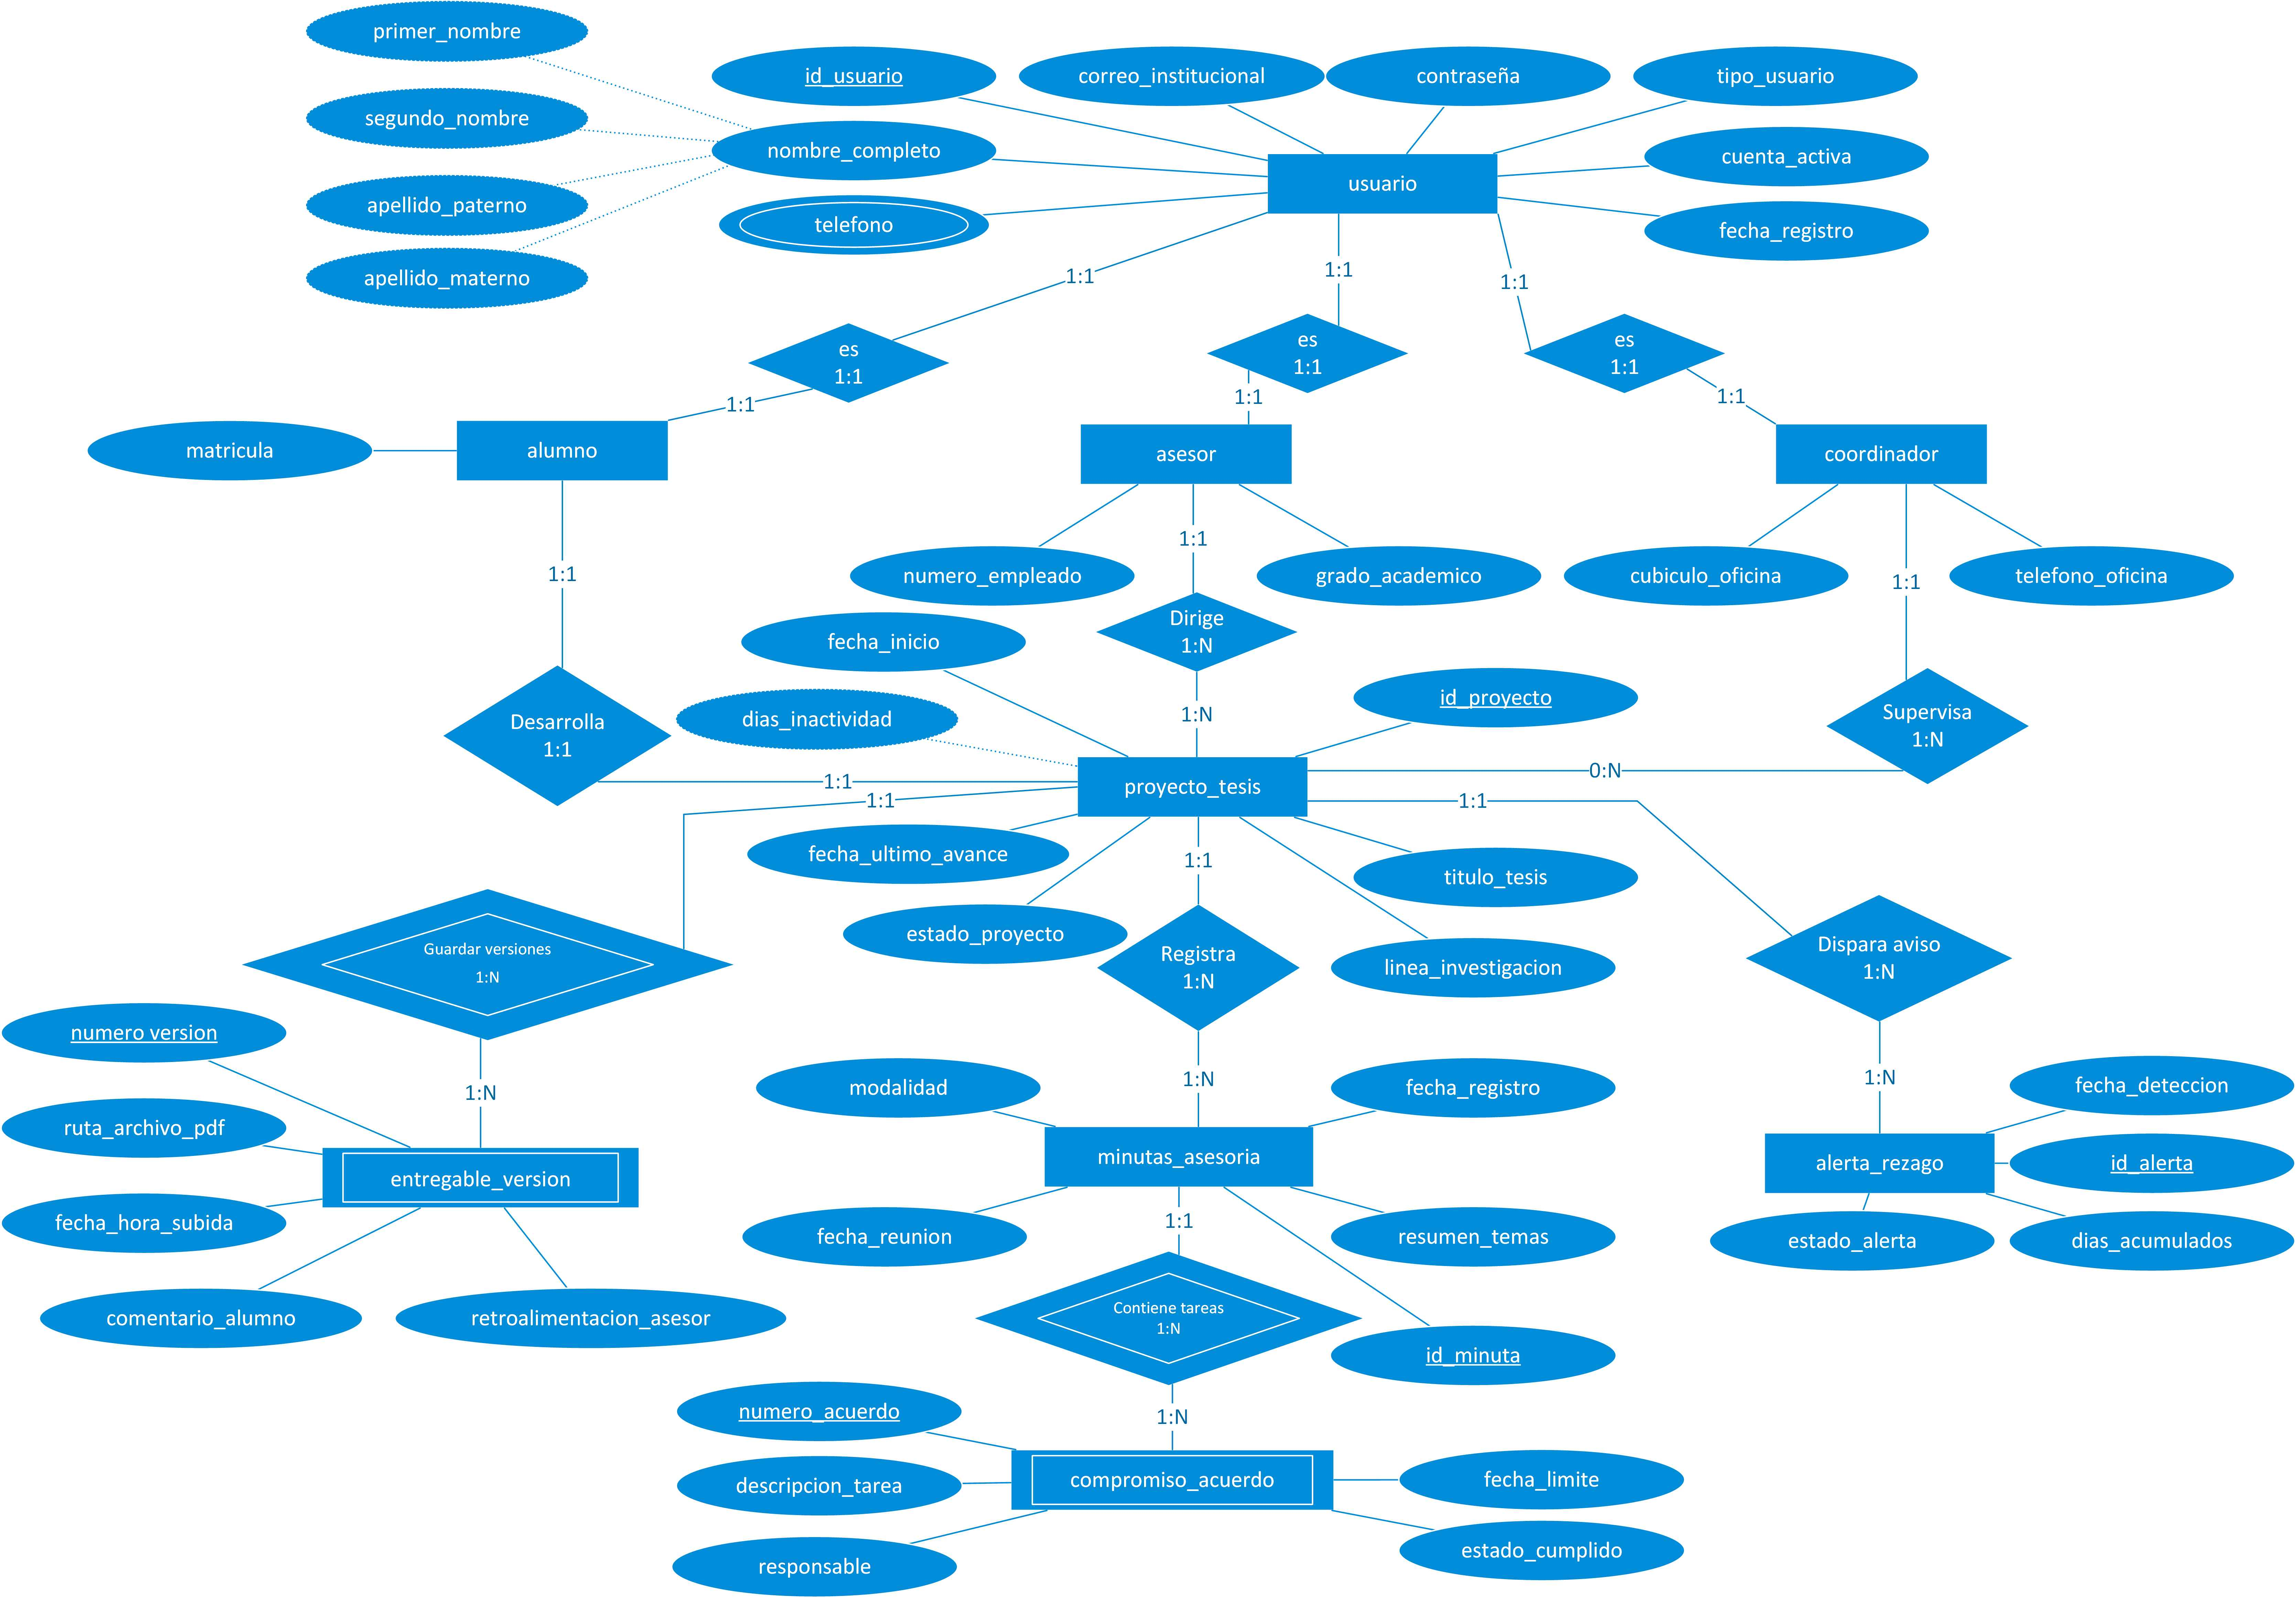
\includegraphics[width=0.95\linewidth]{assets/database/db-MER.jpg}
    \caption{Diagrama Entidad--Relación Extendido de la base de datos.}
    \label{fig:diagrama_eer}
\end{figure}

\subsection{Proceso de Normalización: El Orden de los Datos (1FN, 2FN y 3FN)}
\label{subsec:normalizacion}

Tener el plano visual no es suficiente; si metemos los datos directamente sin revisarlos, corremos el riesgo de duplicar textos, gastar memoria de más o generar errores al intentar actualizar un teléfono. Para solucionar esto se utilizó una técnica llamada \textbf{normalización}. 

En palabras sencillas, normalizar es como vaciar una mochila escolar desordenada para clasificar todo en bolsas y compartimentos específicos: los lápices en la lapicera, los libros en la bolsa grande y la credencial en la bolsa pequeña. Este proceso se realizó en tres pasos continuos:

\subsubsection{Primera Forma Normal (1FN): Datos atómicos y sin amontonar}
La Primera Forma Normal establece que cada celda de una tabla debe guardar un solo dato básico que no se pueda dividir más (valor atómico), prohibiendo meter listas completas en un mismo espacio.

\begin{itemize}
    \item \textbf{Separación de nombres:} En lugar de guardar ``Juan Carlos Pérez López'' en un solo renglón largo, se dividió en primer nombre, segundo nombre, apellido paterno y apellido materno. Gracias a esto, la computadora puede ordenar las listas por orden alfabético de apellidos de manera instantánea.
    \item \textbf{Separación de teléfonos:} Si un estudiante tiene número de celular y número de casa, no se guardan amontonados con comas en una misma celda. Se trasladaron a una tabla independiente (\texttt{telefono\_usuario}), donde cada número ocupa su propio renglón conectado a la persona correspondiente.
    \item \textbf{Tareas individuales:} En las juntas de asesoría no se redactan todos los compromisos en un solo párrafo; cada tarea se registra por separado con su propia fecha límite.
\end{itemize}

\subsubsection{Segunda Forma Normal (2FN): Cada dato depende de su credencial completa}
La Segunda Forma Normal pide que la tabla ya cumpla la 1FN y que todos los datos descriptivos dependan de la credencial o identificador principal completo, no solo de un pedazo. Esto es especialmente importante en tablas que dependen de otras:

\begin{itemize}
    \item \textbf{Entregas de tesis (\texttt{entregable\_version}):} Cada entrega se identifica conjuntamente por el número de proyecto y su número de versión ($v_1, v_2, \dots$). La ruta del PDF, los comentarios y la fecha en que se subió dependen exactamente de esa versión específica de ese trabajo, y no del proyecto en general.
    \item \textbf{Compromisos de reunión (\texttt{compromiso\_acuerdo}):} Cada acuerdo se reconoce por la minuta donde se tomó y el número de tarea asignado. La persona responsable y la fecha de entrega dependen puntualmente de esa tarea acordada.
\end{itemize}

\subsubsection{Tercera Forma Normal (3FN): Cero información ajena o repetida}
La Tercera Forma Normal exige que ningún dato dependa de otra columna que no sea la clave principal. En términos prácticos, significa evitar el ``chisme de pasillo'': ninguna tabla debe guardar datos ajenos que ya le pertenecen por derecho a otra tabla.

\begin{itemize}
    \item \textbf{Separar personas de los proyectos:} En la tabla de tesis no se vuelven a escribir el correo, el teléfono o los nombres del alumno ni del maestro. Únicamente se apunta su número de identificación (\texttt{id\_alumno} e \texttt{id\_asesor}), el cual sirve como un puente o flecha conectora hacia la tabla de usuarios.
    \item \textbf{Separar perfiles escolares:} La matrícula solo le importa al alumno, el número de empleado solo al profesor y la oficina solo al coordinador. Por ello, cada dato particular se colocó en su propia tabla especializada, evitando celdas vacías o datos revueltos.
    \item \textbf{Alertas limpias:} La tabla de alertas registra únicamente los días transcurridos y el estado del aviso, enlazándose a la tesis sin duplicar títulos ni fechas que ya existen en el expediente.
\end{itemize}

\subsection{Estructura Final de Tablas y Relación con los Casos de Uso}
\label{subsec:tablas_casos_uso}

Una vez aplicada la normalización, la información queda organizada en tablas definitivas. Cada una de estas tablas existe para responder y hacer posible el funcionamiento de los cuatro casos de uso principales de la plataforma:

\begin{enumerate}
    \item \textbf{Tabla \texttt{usuario} y Perfiles (Soporte al CU01 -- Inicio de sesión y roles):} 
    Controla el acceso al sistema para que nadie entre a funciones que no le corresponden.
    \begin{itemize}
        \item \textbf{Datos almacenados:} Cuenta con un número identificador único irrepetible (\underline{\texttt{id\_usuario}}), correo institucional, contraseña protegida, nombres desglosados, fecha de registro y la bandera de cuenta activa.
        \item \textbf{Preferencias (\texttt{configuracion\_usuario}):} Guarda de manera personalizada si la persona prefiere la pantalla en tema claro u oscuro y qué avisos visuales desea recibir.
        \item \textbf{Teléfonos (\texttt{telefono\_usuario}):} Permite almacenar múltiples números de contacto para un mismo usuario sin saturar la tabla principal.
        \item \textbf{Especialización de roles:} Se conecta con las tablas \texttt{alumno} (matrícula escolar), \texttt{asesor} (número de empleado y grado académico) y \texttt{coordinador} (cubículo y teléfono de oficina), garantizando que al iniciar sesión cada usuario vea su pantalla específica.
    \end{itemize}

    \item \textbf{Tablas \texttt{convocatoria} y \texttt{proyecto\_tesis} (Expediente académico):}
    Representa la carpeta digital oficial de la investigación y los periodos escolares abiertos por la escuela.
    \begin{itemize}
        \item \textbf{Convocatoria:} Registra las fechas oficiales de apertura, entrega de protocolo y cierre de trámites.
        \item \textbf{Proyecto de tesis:} Guarda el título de la investigación, la línea temática, el protocolo original en PDF, el estado del trabajo y la fecha de inicio.
        \item \textbf{Control de inactividad (Soporte al CU04):} Guarda el dato \texttt{fecha\_ultimo\_avance}. A partir de este registro, el sistema resta automáticamente el día de hoy menos la fecha del último avance, sabiendo cuántos días de inactividad lleva el tesista sin necesidad de cálculos manuales.
        \item \textbf{Conexiones:} Se enlaza directamente con el estudiante titular ($1:1$), el docente asesor ($1:N$) y la coordinación que supervisa ($1:N$).
    \end{itemize}

    \item \textbf{Tablas \texttt{entregable\_version} y \texttt{mensaje\_entrega} (Soporte al CU02 -- Avances en PDF):}
    Permite a los alumnos entregar sus borradores conservando el historial completo de cambios.
    \begin{itemize}
        \item \textbf{Versiones inmutables:} Cada nuevo documento subido recibe un número consecutivo ($v_1, v_2, v_3, \dots$), impidiendo que una entrega nueva borre o sobreescriba un archivo anterior. Almacena la ruta del PDF, la hora exacta de carga y las notas del estudiante.
        \item \textbf{Mensajes de revisión:} Ofrece un canal de comunicación donde el asesor redacta observaciones detalladas sobre ese borrador específico.
    \end{itemize}

    \item \textbf{Tablas \texttt{minutas\_asesoria}, \texttt{compromiso\_acuerdo} y Materiales (Soporte al CU03):}
    Formaliza los acuerdos pactados en las sesiones de trabajo presenciales o virtuales.
    \begin{itemize}
        \item \textbf{Minuta de reunión:} Registra la fecha de la cita, la modalidad, los temas discutidos y las firmas de conformidad.
        \item \textbf{Compromisos de trabajo:} Guarda cada tarea pendiente, indicando quién debe resolverla (el alumno o el docente), la fecha límite obligatoria y una casilla de verificación para marcarla como cumplida.
        \item \textbf{Material de apoyo:} Permite adjuntar lecturas complementarias o artículos recomendados durante la asesoría.
    \end{itemize}

    \item \textbf{Tabla \texttt{alerta\_rezago} (Soporte al CU04 -- Detección de inactividad):}
    Registra los avisos automáticos cuando un estudiante interrumpe su avance.
    \begin{itemize}
        \item \textbf{Datos guardados:} Registra la fecha en que se detectó el retraso, el número exacto de días acumulados y el estado del aviso (pendiente o resuelto).
        \item \textbf{Regla del sistema:} Si el contador supera los 30 días naturales sin registrar nuevos borradores ni minutas de reunión, la tabla guarda un registro que enciende de inmediato un aviso en el panel del profesor y del coordinador.
    \end{itemize}
\end{enumerate}

\subsection{Esquema y Diagrama Relacional Final}
\label{subsec:esquema_relacional}

Una vez superadas las tres formas normales y definidas las funciones de cada tabla, el modelo conceptual se convierte en una base de datos relacional definitiva. En este formato físico, las entidades se convierten en tablas con filas y columnas donde cada conexión se realiza mediante dos tipos de identificadores:

\begin{itemize}
    \item \textbf{Llave Primaria (PK):} Es el número de credencial o folio único de cada renglón que no puede repetirse jamás (por ejemplo, el número único de un usuario o el folio de una minuta).
    \item \textbf{Llave Foránea (FK):} Es una copia de una llave primaria colocada en otra tabla para funcionar como un puente. Gracias a ella, el sistema sabe de inmediato a qué estudiante le pertenece un PDF o a qué reunión corresponde una tarea, sin tener que volver a escribir nombres ni textos repetidos.
\end{itemize}

En la Figura~\ref{fig:diagrama_relacional} se presenta el esquema relacional resultante, mostrando la totalidad de las tablas, sus columnas, los tipos de datos que manejan y las líneas conectoras que aseguran la integridad de la plataforma.

\begin{figure}[htbp]
    \centering
    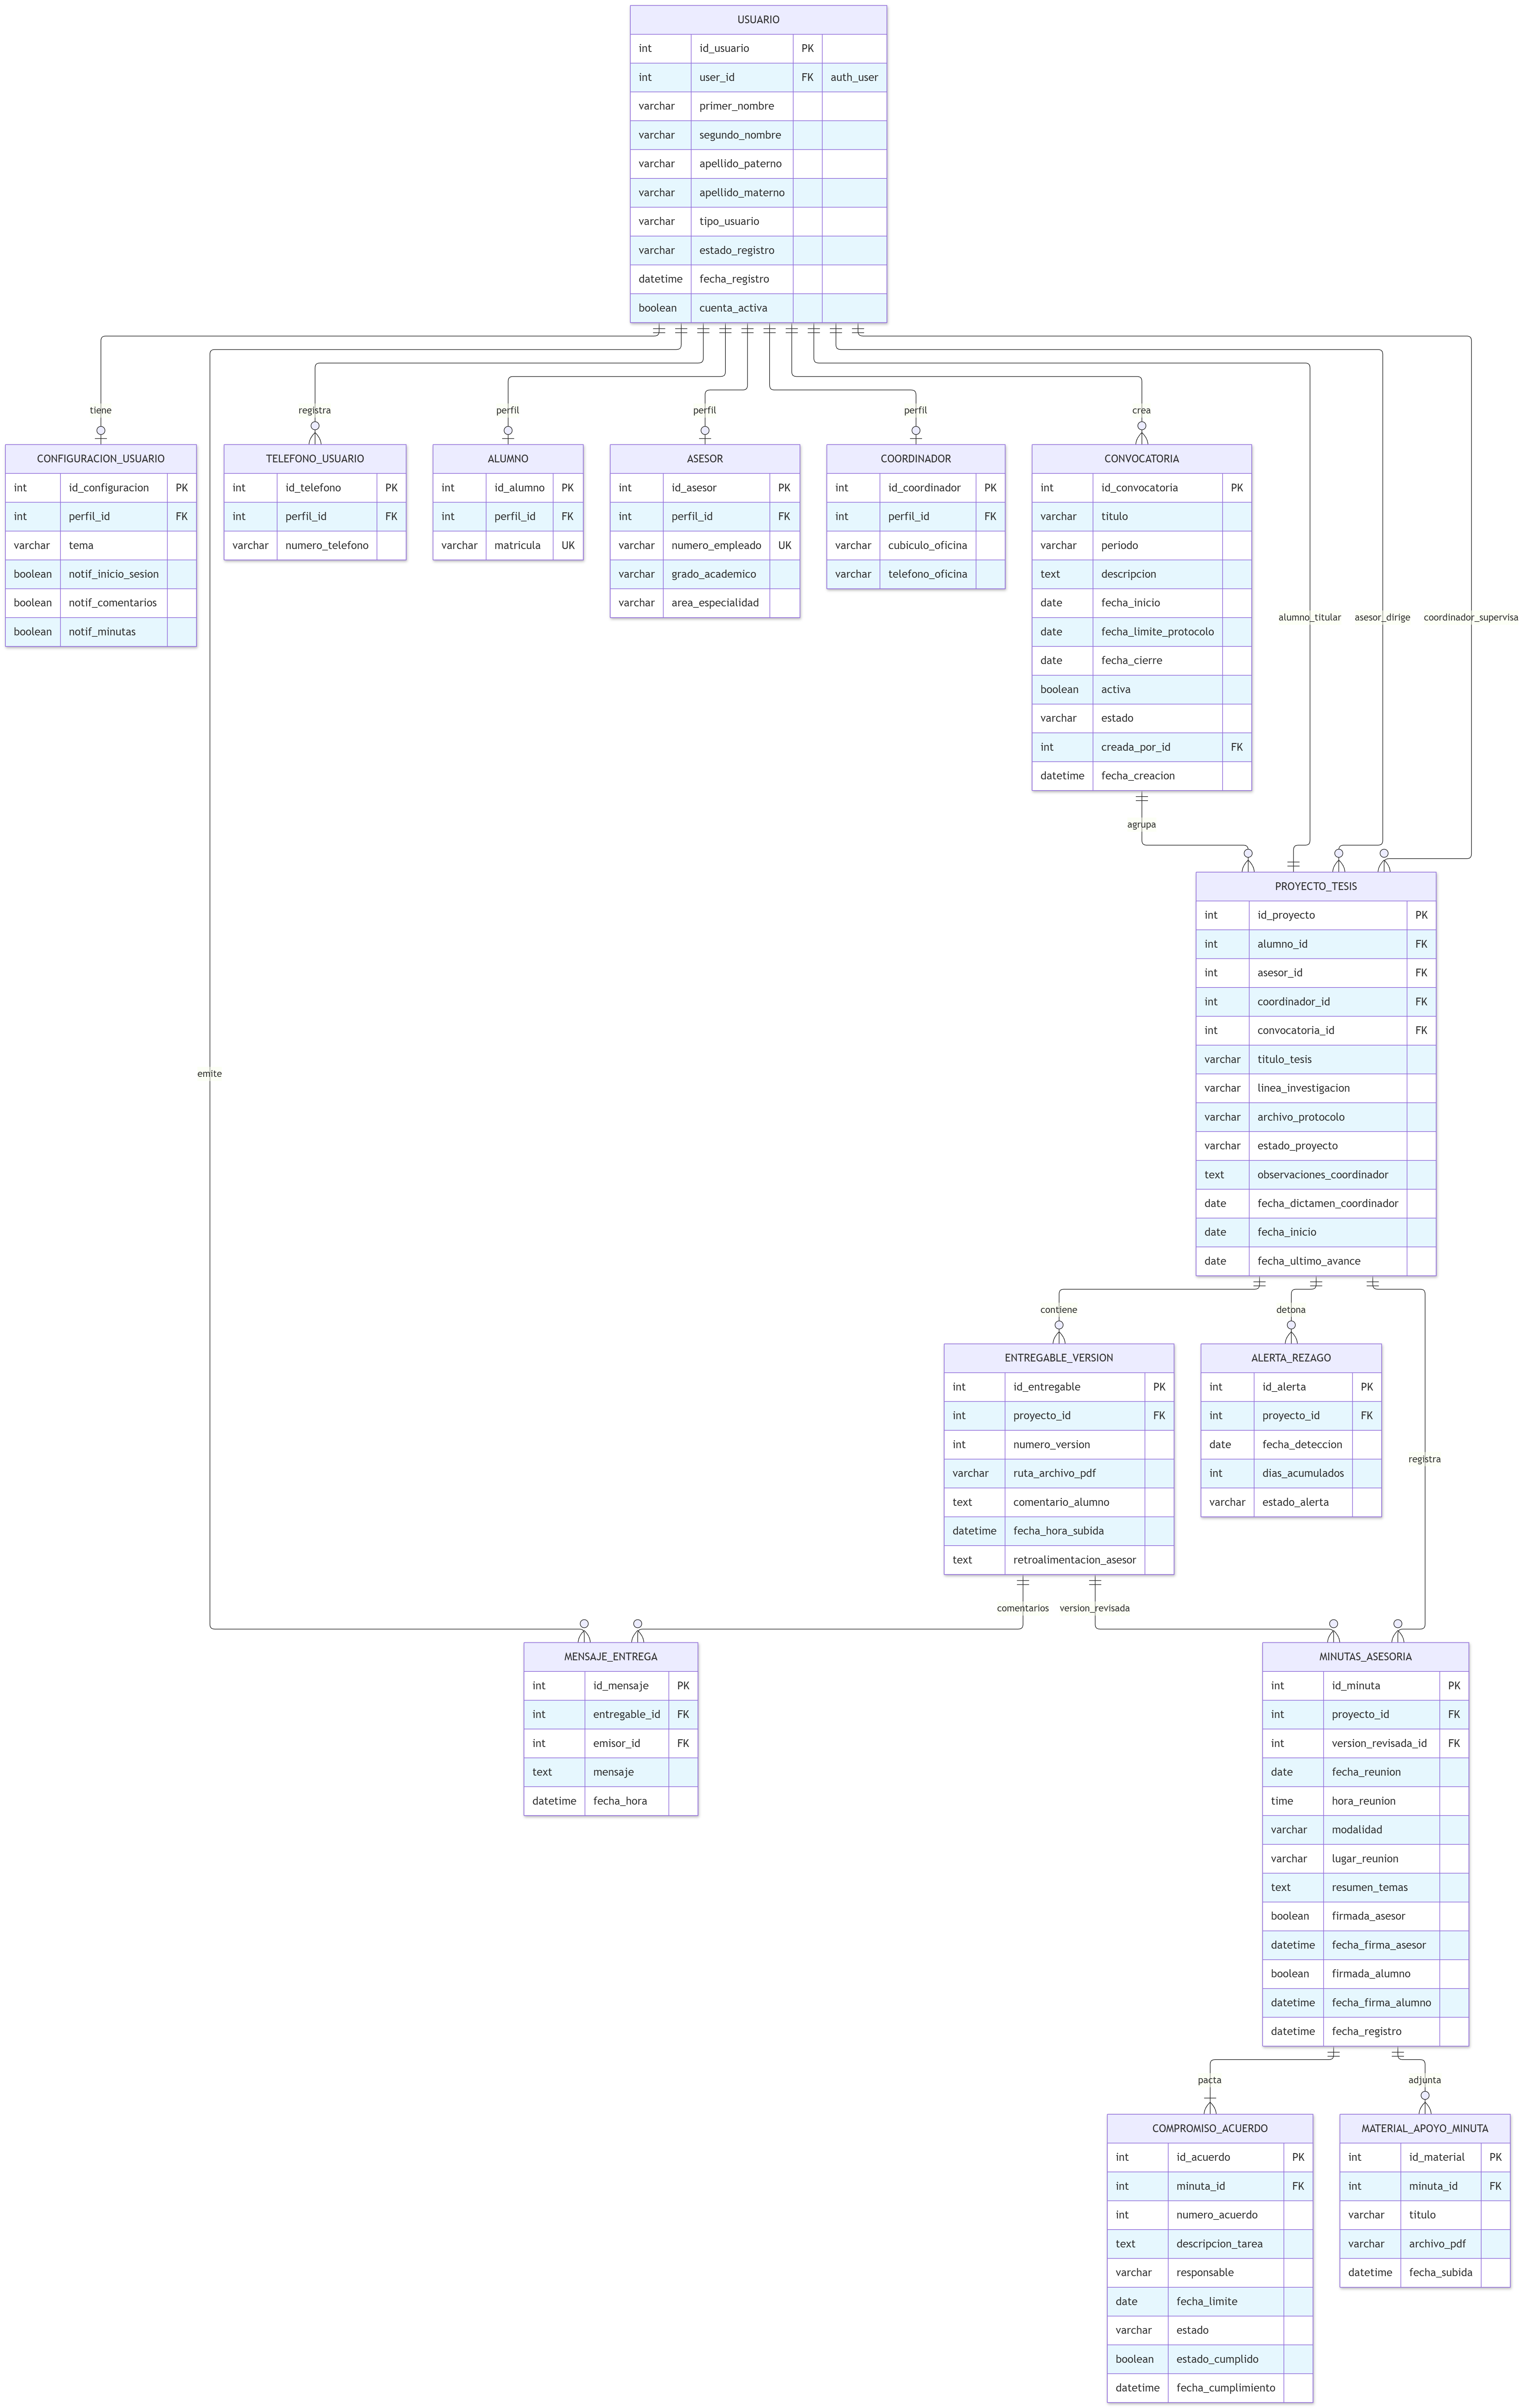
\includegraphics[width=0.8\linewidth]{assets/database/DataBase.png}
    \caption{Diagrama Relacional de la base de datos con tablas, tipos de datos y llaves de unión.}
    \label{fig:diagrama_relacional}
\end{figure}

Con esta estructura organizada, limpia y normalizada, la base de datos garantiza que las consultas sean rápidas, que ningún documento se pierda y que la información permanezca protegida y disponible para toda la comunidad académica.